\section{Contract Net Protocol}

\begin{frame}
	\frametitle{}
	
	\Huge
	
	\vspace{0.5cm}
	
	\begin{center}
		\textbf{Contract Net Protocol}
	\end{center}
\end{frame}

\begin{frame}
	\frametitle{Contract Net Protocol (recap)}
	
	\Large
	
	\begin{itemize}
		\item \emph{Manager} and \emph{Suppliers} communicate via \textbf{offers}
		\vspace{-0.1cm}
		\item Single-manager or Multi-manager
		
		\item Contract specification language:
			  \begin{itemize}
				  \item Requirements, format and deadline for presentation
			  \end{itemize}
		
		\item \textcolor{darkgreen}{Simple and easy to implement}
		
		\item \textcolor{darkgreen}{Dynamic and easily adaptable}
			  \begin{itemize}
			  	  \item \textcolor{darkgreen}{Bilateral contract between manager(s) and supplier(s)}
			  \end{itemize}
		
		\item \textcolor{red}{Many messages}
		\vspace{-0.1cm}
		\item \textcolor{red}{Synchronization problems}
		
		\item \textcolor{red}{Agent behavior:}
			  \begin{itemize}
			  	  \item \textcolor{red}{Cautions, brave or moderate agents}
			  \end{itemize}
	\end{itemize}
\end{frame}

\begin{frame}
	\frametitle{CNP: Single Manager (recap)}
	
	\Large
	
	\vspace{0.2cm}
	
	How to get a contract:
	
	\begin{itemize}
		\item \textbf{Announcement: } manager \emph{sends} the task description to all the
			  possible suppliers
		\vspace{0.1cm}
		\item \textbf{Bidding: } suppliers \emph{evaluate} the offer and send a proposal to
			  the manager
		\vspace{0.1cm}
		\item \textbf{Awarding: } manager \emph{evaluates} the proposals and allocates the
			  contract to the best suppliers
		\vspace{0.1cm}
		\item \textbf{Expediting: } the chosen suppliers \emph{accepts} or \emph{rejects}
			  the assignment
	\end{itemize}
\end{frame}

\begin{frame}
	\frametitle{CNP: Example}
	
	\Large
	
	\begin{itemize}
		\item Consider the problem of $ N $ robotic agents willing to cook a pie:
			  
			  \begin{itemize}
			  	  \item They have to collect ingredients, then meet in the home location
						$ H $ to prepare the pie
				  \vspace{0.05cm}
				  \item The agents start cooperating at time $ I $, and have to meet in the
						home location at time $ T $
			  \end{itemize}
		
		\item Each agent is initially given the assignment to buy a certain ingredient
		
		\item Each agent must make sure to complete its tasks and arrive to the home
			  location before time $ T $
	\end{itemize}
\end{frame}

\begin{frame}
	\frametitle{CNP: Example - cont'd}
	
	\Large
	
	\vspace{0.4cm}
	
	\begin{itemize}
		\item Each agent uses Manhattan distances (in a world represented by a uniform
			  grid) to know the time needed to reach each destination
		
		\item Time needed by agents to exchange messages for coordination is negligible
	\end{itemize}
	
	\vspace{-0.35cm}
	
	\begin{figure}[!t]
		\centering
		\vspace{0.2cm}
		\begin{tikzpicture}[map/.style={draw=white,ultra thick,inner sep=0pt}]
			\node at (0,0) [map]
			{
				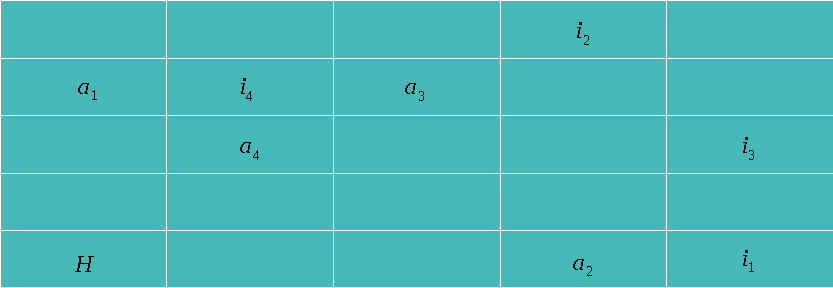
\includegraphics[width=0.85\linewidth]{Figures/Grid}
			};
		\end{tikzpicture}
	\end{figure}
\end{frame}

\begin{frame}
	\frametitle{CNP: Example - cont'd}
	
	\Large 
	
	\begin{enumerate}
		\item Describe a simple CNP to let agents reach the goal of preparing the pie -
			  assume to have all ingredients in the home location on time
			  
			  \begin{itemize}
				  \item It is not requested that the protocol always reaches the solution -
						if it exists - but it has to always terminates either with an
						assignment or with a failure. If possible, show the pseudo-code
						executed by the agents
			  \end{itemize}
		
		\item Provide a possible execution of the coordination protocol, and the final
			  assignment of agents and ingredients, assuming that:
			  
			  \begin{itemize}
			  	  \item There are $ N = 4 $ and the meeting time is at time $ T = 10 $
			  	  
			  	  \item Agents and ingredients are located as shown in the previous figure
			  	  
			  	  \item Agent $ a_j $ is initially in charge of buying ingredient $ i_j $
						(e.g., $ a_1 $ buys $ i_1 $)
			  \end{itemize}
	\end{enumerate}
\end{frame}

\begin{frame}
	\frametitle{CNP: Example Solution}
	
	\vspace{0.3cm}
	
	These can be the settings to reach an agreement:
	
	\begin{itemize}
		\item Agents who are not able to reach home in time, due to their current
			  assignments, start the CNP on the most inconvenient task, in order to let it
			  be performed by other agents (they are the managers)
		\vspace{0.1cm}
		\item The policy to make proposals is the Manhattan distance between the initial
			  position and the destination
		\vspace{0.1cm}
		\item An agent is not interested if that task would not let him reach home in time,
			  and if it would reach an assignment already reached in the past
		\vspace{0.1cm}
		\item Agents do not schedule their tasks when proposing (brave agents)
		\vspace{0.1cm}
		\item If an agent is not able to complete its tasks in time, neither to give it to
			  someone else through CNP, declares the failure of the protocol
	\end{itemize}
\end{frame}

\begin{frame}
	\frametitle{CNP: Example Solution - cont'd}
	
	\begin{itemize}
		\item $ a_1 $ starts CNP for $ i_1 $, receiving proposals $ \langle HNR,1,5,5
			  \rangle $ and \textcolor{red}{assigning the task to $ a_2 $}
		
		\item $ a_2 $ starts CNP for $ i_2 $, receiving proposals $ \langle HNR,HNR,2,HNR
			  \rangle $ and \textcolor{red}{assigning the task to $ a_3 $}
		
		\item Since $ a_3 $ is assigned with $ i_2 $ and $ i_3 $, it will start CNP for $
			  i_3 $ receiving proposals $ \langle HNR,3,3,3 \rangle $ and \textcolor{red}
			  {assigning the task - for example - to $ a_2 $}
		
		\item Since $ a_2 $ is now assigned with $ i_1 $ and $ i_3 $, it will start CNP for
			  $ i_3 $ again, receiving proposals $ \langle HNR,AA,AA,3 \rangle $ and
			  \textcolor{red}{assigning the task to $ a_4 $}
		
		\item Since $ a_4 $ is now assigned with $ i_3 $ and $ i_4 $, it will start CNP for
			  $ i_3 $ \textcolor{red}{receiving no answers}
		
		\item So, it starts CNP for $ i_4 $ receiving proposals $ \langle 1,AA,AA,AA
			  \rangle $ \textcolor{red}{assigning the task to $ a_1 $}
		
		\item The final assignment will be $ \langle a_1,i_4 \rangle, \langle a_2,i_1
			  \rangle, \langle a_3,i_2 \rangle, \langle a_4,i_1 \rangle$
	\end{itemize}
\end{frame}

\begin{frame}
	\frametitle{CNP: Example Solution - cont'd}
	
	\Large
	
	\vspace{0.2cm}
	
	However, the assignment is not optimal because:
	
	\begin{itemize}
		\item If the initial assignment was able to let each agent reach the home
			  destination in time - but with inconvenient paths - none would start the
			  coordination
		
		\item Each iteration of CNP requires $ N + 2 $ messages
		
		\item Number of messages is quadratic in the number of agents
		
		\item CNP is executed at most $ N $ times for each task, to assign different
			  winners every time
	\end{itemize}
\end{frame}

\begin{frame}
	\frametitle{CNP: Exercise}
	
	\vspace{0.3cm}
	
	Agents and domain: each agent controls one sensor as depicted in the figure:
	
	\begin{figure}[!t]
		\centering
		\vspace{-0.2cm}
		\begin{tikzpicture}[map/.style={draw=white,ultra thick,inner sep=0pt}]
			\node at (0,0) [map]
			{
				\includegraphics[width=0.58\linewidth]{Figures/Exercise}
			};
		\end{tikzpicture}
	\end{figure}
\end{frame}

\begin{frame}
	\frametitle{CNP: Exercise - cont'd}
	
	\Large
	
	\begin{itemize}
		\item $ S_i $ may turn on only one slot at each time instance
		
		\item $ \langle S_{ij},t_k \rangle $: slot $ j $ of sensor $ i $ is turned on at
			  time $ t_k $
		
		\item In order to detect a vehicle, two sensors at least have to observe the
			  vehicle in a maximum temporal window of $ X $ time instances after the first
			  detection
		
		\item False detections are possible: the second sensor does not perceive the
			  vehicle when it was first detected by the other sensor
	\end{itemize}
\end{frame}

\begin{frame}
	\frametitle{CNP: Exercise - cont'd}
	
	\large
	
	\vspace{0.3cm}
	
	\textbf{Goal:} \emph{verify} the maximum possible number of vehicles
	
	\vspace{0.3cm}
	
	\textbf{Specifications:}
	
	\begin{itemize}
		\item One agent cannot accomplish the goal alone: the agents must cooperate to turn
			  on their slots and verify the vehicle
		\vspace{0.1cm}
		\item Use CNP multi-manager protocol to solve this problem, letting the agent take
			  meeting times for vehicle verifications
		\vspace{0.1cm}
		\item Show the execution of the protocol starting from the initial situation $
			  on(S_{13}), on(S_{23}), on(S_{31}), t = 1 $
		\vspace{0.1cm}
		\item Study performance of the protocol in terms of optimality, waiting times and
			  number of messages needed
	\end{itemize}
\end{frame}

\begin{frame}
	\frametitle{CNP: Exercise Solution}
	
	\Large
	
	\vspace{0.3cm}
	
	\begin{itemize}
		\item The agent who perceives the vehicle in position $ \langle x,y \rangle $
			  becomes the manager and broadcasts request for actions for undetected $
			  \langle x,y \rangle $
		\vspace{0.1cm}
		\item It will accept the earliest proposal
		\vspace{0.1cm}
		\item Only interested agents answers: each agent who is able to schedule a meeting
			  time, offers the first free time slot
		\vspace{0.1cm}
		\item Agents who proposed a meeting time during the CNP and wins, cannot refuse its
			  proposal
	\end{itemize}
\end{frame}

\begin{frame}
	\frametitle{CNP: Exercise Solution - cont'd}
	
	\vspace{0.3cm}
	
	\begin{algorithm}[H]
		\caption{EndBidChecker}
		\BlankLine
		$ checkEndBids(); $ \\
		\BlankLine
		\For {\textbf{all} $ endBidTime(ok) $}
		{
			$ (a_i,t_j) = selectWinner(); $ \\
			$ schedule(s(ok),t_j); $ \\
			$ sendAccept(ok,a_i);$ \\
			\BlankLine
			\For {\textbf{all} $ a_l \neq a_i $}
			{
				$ sendRefusal(ok,a_l) $
			}
		}
	\end{algorithm}
\end{frame}

\begin{frame}
	\frametitle{CNP: Exercise Solution - cont'd}
	
	\vspace{0.3cm}
	
	\begin{algorithm}[H]
		\caption{MsgBoxChecker}
		\BlankLine
		$ checkMsgBox(); $ \\
		\BlankLine
		\For {\textbf{all} $ msgReceived $ $ m $}
		{
			\uIf {$ m = req(ok,a_i,t_{bid},[t_{min},t_{max}]) $}
			{
				$ sendProposal(ok,a_i,firstFree([t_{min},t_{max}])); $
			}
			\ElseIf {$ m = accept(ok,a_i,t_{task}) $}
			{
				$ schedule(s(ok),t_{task}); $
			}
		}
	\end{algorithm}
\end{frame}

\begin{frame}
	\frametitle{CNP: Exercise Solution - cont'd}
	
	\vspace{0.3cm}
	
	\begin{algorithm}[H]
		\caption{NewObjectChecker}
		\BlankLine
		$ checkNewObjects(); $ \\
		$ s_i = chooseBestSector(); $ \\
		\BlankLine
		\For {\textbf{all} $ ok \in o(s_i) $}
		{
			$ t_m = firstFree(t_{cur} + 2,\infty); $ \\
			$ broadcastRequest(ok,t_{bid} = t_{cur} + 1,[t_m,t_m + 3]); $
		}
		\BlankLine
		\If {$ scheduled(t_{cur}) $}
		{
			$ turnOn(scheduledSector(t_{cur})); $
		}
	\end{algorithm}
\end{frame}

\begin{frame}
	\frametitle{CNP: Exercise Execution}
	
	Initial state: $ on(S_{13}), \; on(S_{23}), \; on(S_{31}), \; t = 1 $ \\
	
	\vspace{0.4cm}
	
	$ \mathbf{A_1:} $ $ broadcastRequest(o_1,A_1,t_2,[t_3,t_6]) $ \\
	$ \;\;\;\;\;\,\,\,\, broadcastRequest(o_2,A_1,t_2,[t_3,t_6]) $ \\
	
	\vspace{0.1cm}
	
	$ \mathbf{A_2:} $ $ receives $ $ m = req(o_1,A_1,t_2,[t_3,t_6]) \rightarrow sendProposal(o_1,A_1,t_3) $ \\
	$ \;\;\;\;\;\,\,\,\, receives $ $ m = req(o_2,A_1,t_2,[t_3,t_6]) \rightarrow sendProposal(o_2,A_1,t_3) $ \\
	$ \;\;\;\;\;\,\,\,\, broadcastRequest(o_3,A_2,t_2,[t_4,t_7]) $ \\
	$ \;\;\;\;\;\,\,\,\, broadcastRequest(o_4,A_2,t_2,[t_4,t_7]) $ \\
	
	\vspace{0.1cm}
	
	$ \mathbf{A_3:} $ $ receives $ $ m = req(o_1,A_1,t_2,[t_3,t_6]) \rightarrow sendProposal(o_1,A_1,t_3) $ \\
	$ \;\;\;\;\;\,\,\,\, receives $ $ m = req(o_2,A_1,t_2,[t_3,t_6]) \rightarrow sendProposal(o_2,A_1,t_4) $ \\
	$ \;\;\;\;\;\,\,\,\, receives $ $ m = req(o_3,A_2,t_2,[t_4,t_7]) \rightarrow sendProposal(o_3,A_2,t_4) $ \\
	$ \;\;\;\;\;\,\,\,\, receives $ $ m = req(o_4,A_2,t_2,[t_4,t_7]) \rightarrow sendProposal(o_4,A_2,t_5) $ \\
	
	\vspace{0.1cm}
	
	$ t = 2 $ \\
\end{frame}

\begin{frame}
	\frametitle{CNP: Exercise Execution - cont'd}
	
	\vspace{0.25cm}
	
	$ \mathbf{A_1:} $ $ endBidTime(o_1) \rightarrow sendAccept(o_1,A_2,t_3) $ \\
	$ \;\;\;\;\;\,\,\,\, sendRefusal(o_1,A_3) $ \\
	$ \;\;\;\;\;\,\,\,\, schedule(S_{13},t3) $ \\
	$ \;\;\;\;\;\,\,\,\, endBidTime(o_2) \rightarrow sendAccept(o_2,A_2,t_3) $ \\
	$ \;\;\;\;\;\,\,\,\, sendRefusal(o_2,A_3) $ \\
	$ \;\;\;\;\;\,\,\,\, receives $ $ m = req(o_3,A_2,t_2,[t_4,t_7]) \rightarrow sendProposal(o_3,A_2,t_4) $ \\
	$ \;\;\;\;\;\,\,\,\, receives $ $ m = req(o_4,A_2,t_2,[t_4,t_7]) \rightarrow sendProposal(o_4,A_2,t_5) $ \\
	
	\vspace{0.1cm}
	
	$ \mathbf{A_2:} $ $ endBidTime(o_3) \rightarrow sendAccept(o_3,A_3,t_4) $ \\
	$ \;\;\;\;\;\,\,\,\, sendRefusal(o_3,A_1) $ \\
	$ \;\;\;\;\;\,\,\,\, schedule(S_{23},t4) $ \\
	$ \;\;\;\;\;\,\,\,\, endBidTime(o_4) \rightarrow sendAccept(o_4,A_3,t_5) $ \\
	$ \;\;\;\;\;\,\,\,\, sendRefusal(o_4,A_1) $ \\
	$ \;\;\;\;\;\,\,\,\, schedule(S_{23},t5) $ \\
	$ \;\;\;\;\;\,\,\,\, receives $ $ m = accept(o_1,A_2,t_3) $ $ and $ \\
	$ \;\;\;\;\;\,\,\,\,\;\;\;\;\;\;\;\;\;\;\;\;\; m = accept(o_2,A_2,t_3) \rightarrow schedule(S_{22},t_3) $ \\
\end{frame}

\begin{frame}
	\frametitle{CNP: Exercise Execution - cont'd}
	
	\vspace{-3cm}
	
	$ \mathbf{A_3:} $ $ receives $ $ m = accept(o_3,A_3,t_4) \rightarrow schedule(S_{33},t_4) $ \\
	$ \;\;\;\;\;\,\,\,\, receives $ $ m = accept(o_4,A_3,t_5) \rightarrow schedule(S_{32},t_5) $ \\
\end{frame}

\begin{frame}
	\frametitle{CNP: Exercise Analysis}
	
	\Large
	
	\textbf{Number of messages:} \\
	
	\begin{center}
		\vspace{-0.1cm}
		
		$ num_{msg} \leq num_{task} \times (3 \times num_{ag}) = o(num_{task} \times
		  num_{ag}) $
	\end{center}
	
	\vspace{0.3cm}
	
	\textbf{Waiting time:} \\	
	
	\begin{center}
		\vspace{-0.1cm}
		
		$ T_{tot} = (bid_{time} + 2) \times T_{msg} + T_{execTask} $
	\end{center}
	
	\vspace{0.4cm}
	
	The retrieved solution is not optimal (trivial)
\end{frame}
